%!TEX root = ../diffusion_paper.tex
\section{Motivation and Aims} % (fold)
\label{sec:motivation_and_aims}
  % The very first letter is a 2 line initial drop letter followed
  % by the rest of the first word in caps.
  % 
  % form to use if the first word consists of a single letter:
  % \IEEEPARstart{A}{demo} file is ....
  % 
  % form to use if you need the single drop letter followed by
  % normal text (unknown if ever used by IEEE):
  % \IEEEPARstart{A}{}demo file is ....
  % 
  % Some journals put the first two words in caps:
  % \IEEEPARstart{T}{his demo} file is ....
  % 
  % Here we have the typical use of a "T" for an initial drop letter
  % and "HIS" in caps to complete the first word.
  \IEEEPARstart{T}{his} demo file is intended to serve as a ``starter file''
  for IEEE journal papers produced under \LaTeX\ using
  IEEEtran.cls version 1.7 and later.
  % You must have at least 2 lines in the paragraph with the drop letter
  % (should never be an issue)
  I wish you the best of success.

  \hfill mds
 
  \hfill January 11, 2007

  \subsection{Subsection Heading Here}
  Subsection text here.

  % needed in second column of first page if using \IEEEpubid
  %\IEEEpubidadjcol

  \subsubsection{Subsubsection Heading Here}
  Subsubsection text here.


  % An example of a floating figure using the graphicx package.
  % Note that \label must occur AFTER (or within) \caption.
  % For figures, \caption should occur after the \includegraphics.
  % Note that IEEEtran v1.7 and later has special internal code that
  % is designed to preserve the operation of \label within \caption
  % even when the captionsoff option is in effect. However, because
  % of issues like this, it may be the safest practice to put all your
  % \label just after \caption rather than within \caption{}.
  %
  % Reminder: the "draftcls" or "draftclsnofoot", not "draft", class
  % option should be used if it is desired that the figures are to be
  % displayed while in draft mode.
  %
  %\begin{figure}[!t]
  %\centering
  %\includegraphics[width=2.5in]{myfigure}
  % where an .eps filename suffix will be assumed under latex, 
  % and a .pdf suffix will be assumed for pdflatex; or what has been declared
  % via \DeclareGraphicsExtensions.
  %\caption{Simulation Results}
  %\label{fig_sim}
  %\end{figure}

  % Note that IEEE typically puts floats only at the top, even when this
  % results in a large percentage of a column being occupied by floats.


  % An example of a double column floating figure using two subfigures.
  % (The subfig.sty package must be loaded for this to work.)
  % The subfigure \label commands are set within each subfloat command, the
  % \label for the overall figure must come after \caption.
  % \hfil must be used as a separator to get equal spacing.
  % The subfigure.sty package works much the same way, except \subfigure is
  % used instead of \subfloat.
  %
  %\begin{figure*}[!t]
  %\centerline{\subfloat[Case I]\includegraphics[width=2.5in]{subfigcase1}%
  %\label{fig_first_case}}
  %\hfil
  %\subfloat[Case II]{\includegraphics[width=2.5in]{subfigcase2}%
  %\label{fig_second_case}}}
  %\caption{Simulation results}
  %\label{fig_sim}
  %\end{figure*}
  %
  % Note that often IEEE papers with subfigures do not employ subfigure
  % captions (using the optional argument to \subfloat), but instead will
  % reference/describe all of them (a), (b), etc., within the main caption.


  % An example of a floating table. Note that, for IEEE style tables, the 
  % \caption command should come BEFORE the table. Table text will default to
  % \footnotesize as IEEE normally uses this smaller font for tables.
  % The \label must come after \caption as always.
  %
  %\begin{table}[!t]
  %% increase table row spacing, adjust to taste
  %\renewcommand{\arraystretch}{1.3}
  % if using array.sty, it might be a good idea to tweak the value of
  % \extrarowheight as needed to properly center the text within the cells
  %\caption{An Example of a Table}
  %\label{table_example}
  %\centering
  %% Some packages, such as MDW tools, offer better commands for making tables
  %% than the plain LaTeX2e tabular which is used here.
  %\begin{tabular}{|c||c|}
  %\hline
  %One & Two\\
  %\hline
  %Three & Four\\
  %\hline
  %\end{tabular}
  %\end{table}


  % Note that IEEE does not put floats in the very first column - or typically
  % anywhere on the first page for that matter. Also, in-text middle ("here")
  % positioning is not used. Most IEEE journals use top floats exclusively.
  % Note that, LaTeX2e, unlike IEEE journals, places footnotes above bottom
  % floats. This can be corrected via the \fnbelowfloat command of the
  % stfloats package.
  
  \begin{figure}[!t]
    \centering
    \subfloat[]{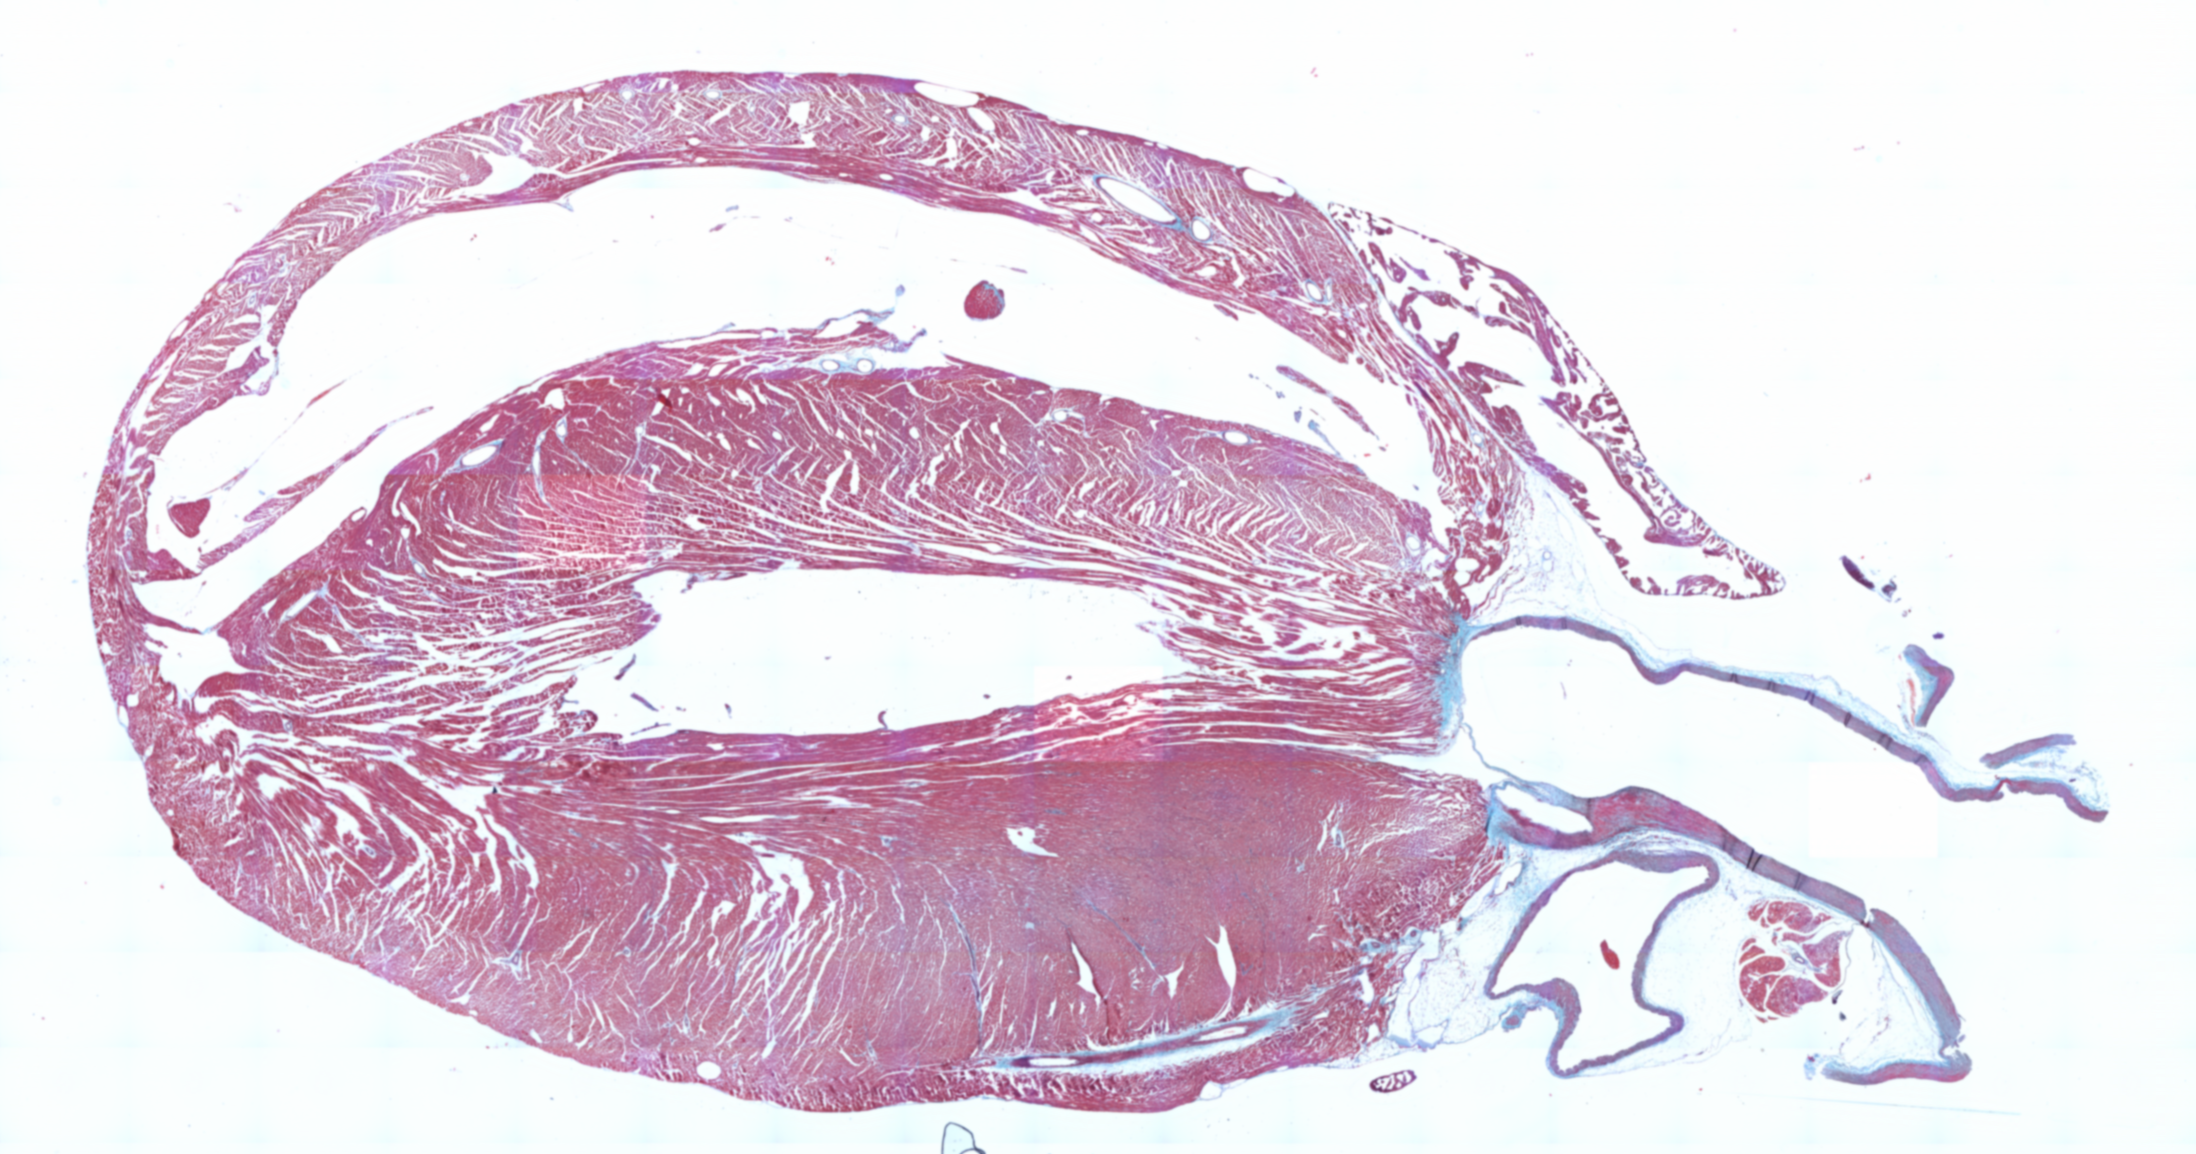
\includegraphics[width=1.7in]{1_motivation_and_aims/Figs/HiRes_downsamples_8_0582}}
    \subfloat[]{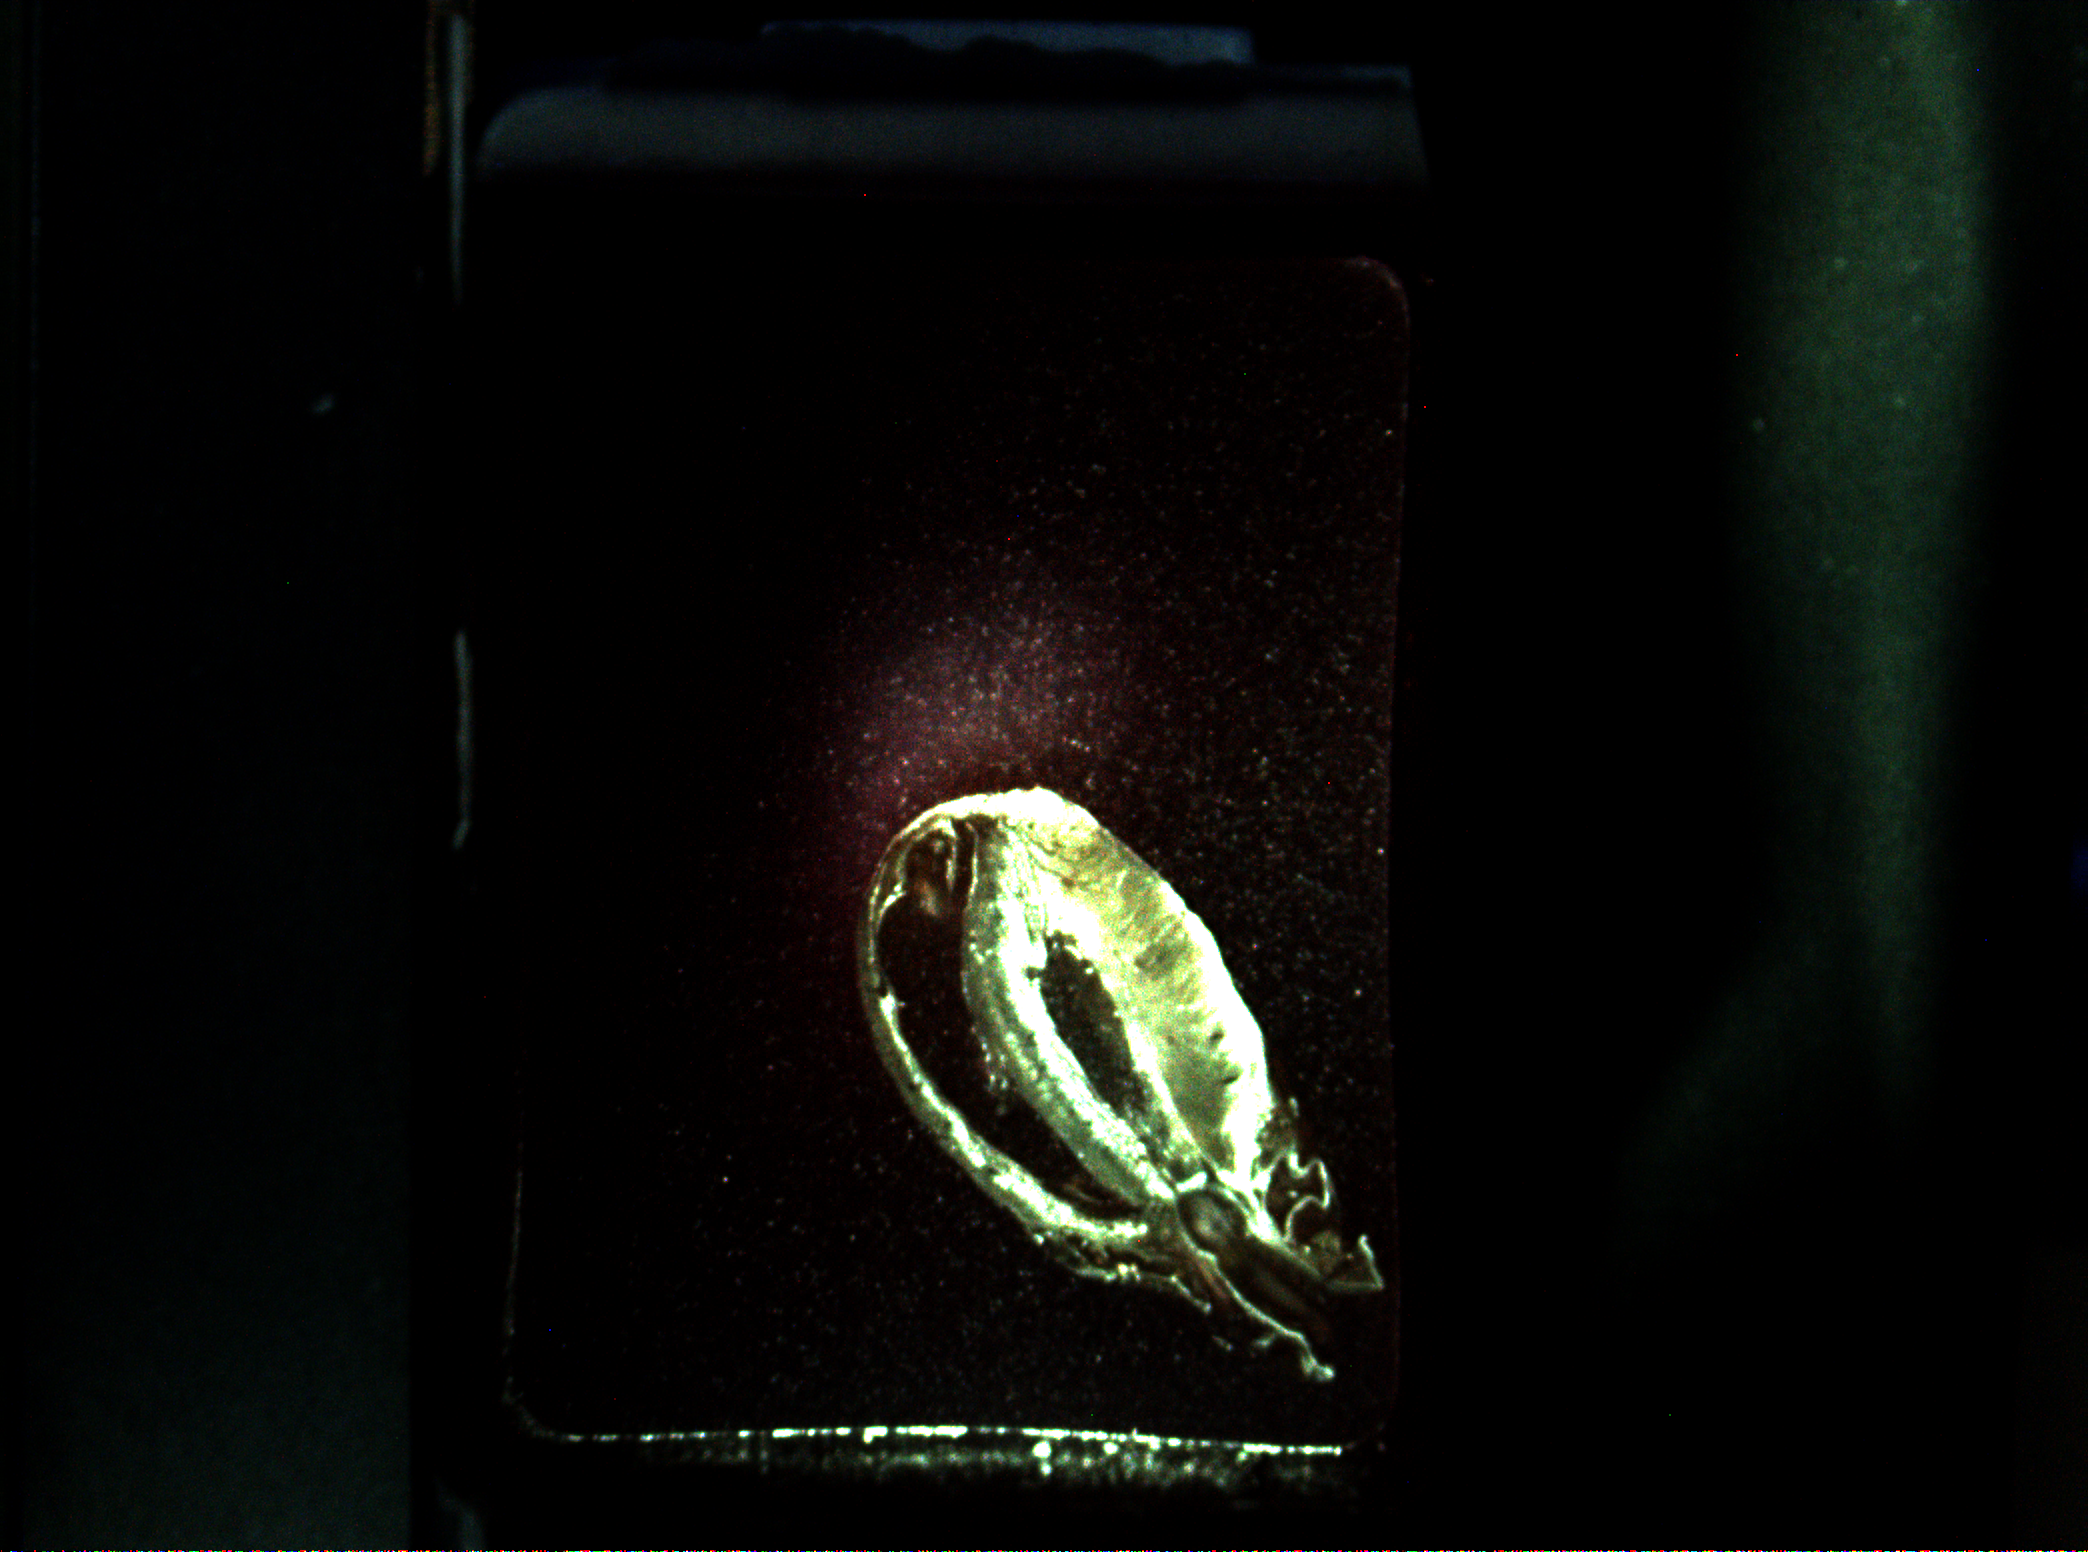
\includegraphics[width=1.7in]{1_motivation_and_aims/Figs/LoRes_rgb_downsamples_1_0582}}\\
    \subfloat[]{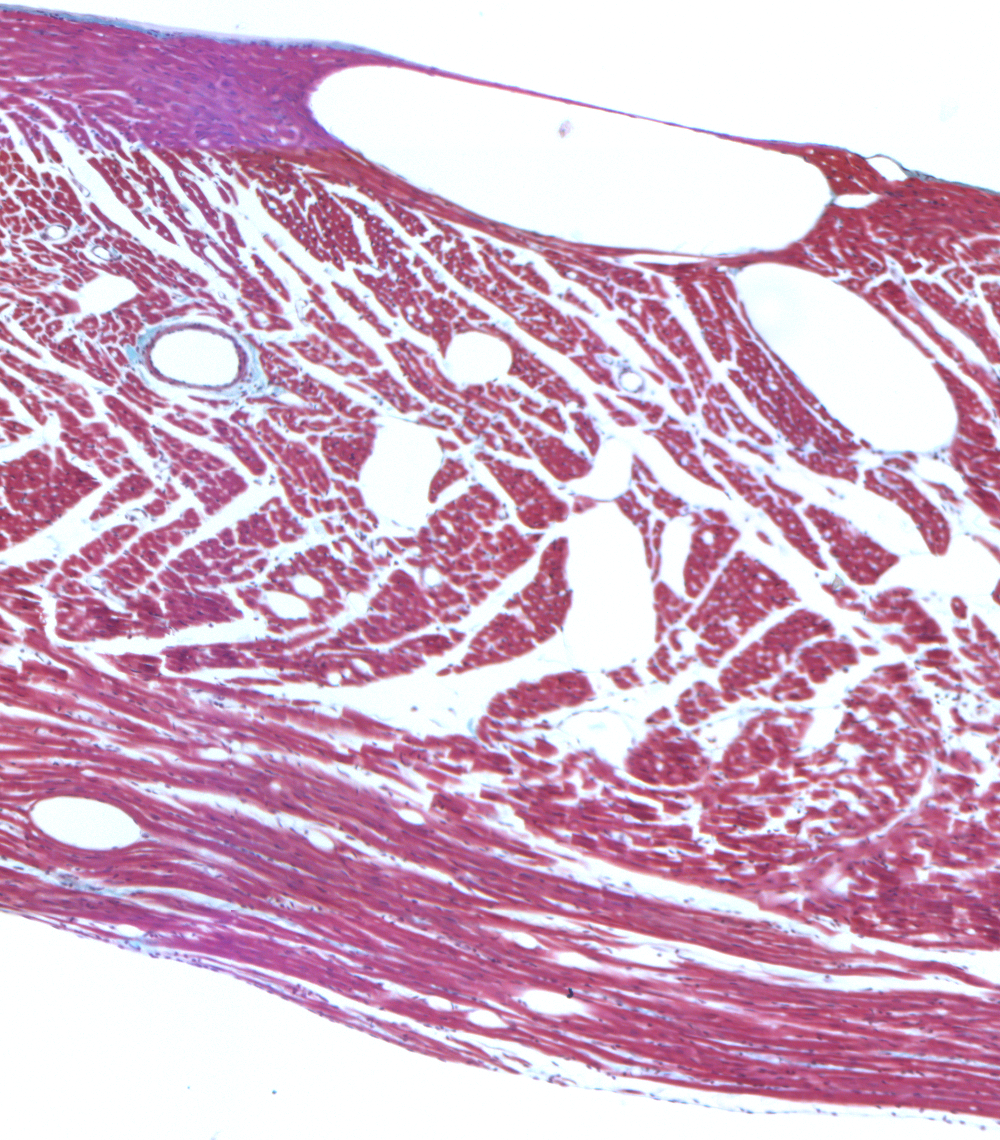
\includegraphics[width=1.7in]{1_motivation_and_aims/Figs/HiRes_downsamples_1_0582_zoom}}
    \subfloat[]{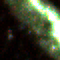
\includegraphics[width=1.7in]{1_motivation_and_aims/Figs/LoRes_rgb_downsamples_1_0582_zoom}}
    \caption{Figure on starting point, showing dataset images, whole and with zoom}
    \label{fig:synthetic_cross_sections}
  \end{figure}
    
  
% section motivation_and_aims (end)
